  Одной из целей эксперимента Belle II является достижение проектной светимости равной $8\cdot10^{35}$с$^{-1}$см$^{-2}$. Такая огромная светимость поставила строгие ограничения на детектор, в связи с чем потребовалось произвести множество улучшений. Также в процессе работы при таких значениях светимости необходимо тщательно контролировать процесс набора данных и иметь обратную связь с ускорителем и детектором для оперативного обнаружения и исправления неисправностей и  настройки оптимальных параметров. Для данной цели используются три онлайн монитора светимости: LumiBelle2, zero degree luminosity monitor (ZDLM) и онлайн монитор светимости (ECL LOM), на улучшение которого и направлена данная работа. Модуль LOM (Рис. 5) был разработан в ИЯФ СО РАН и произведен в 2016 году. 
\begin{figure}[htp]
  \centering
  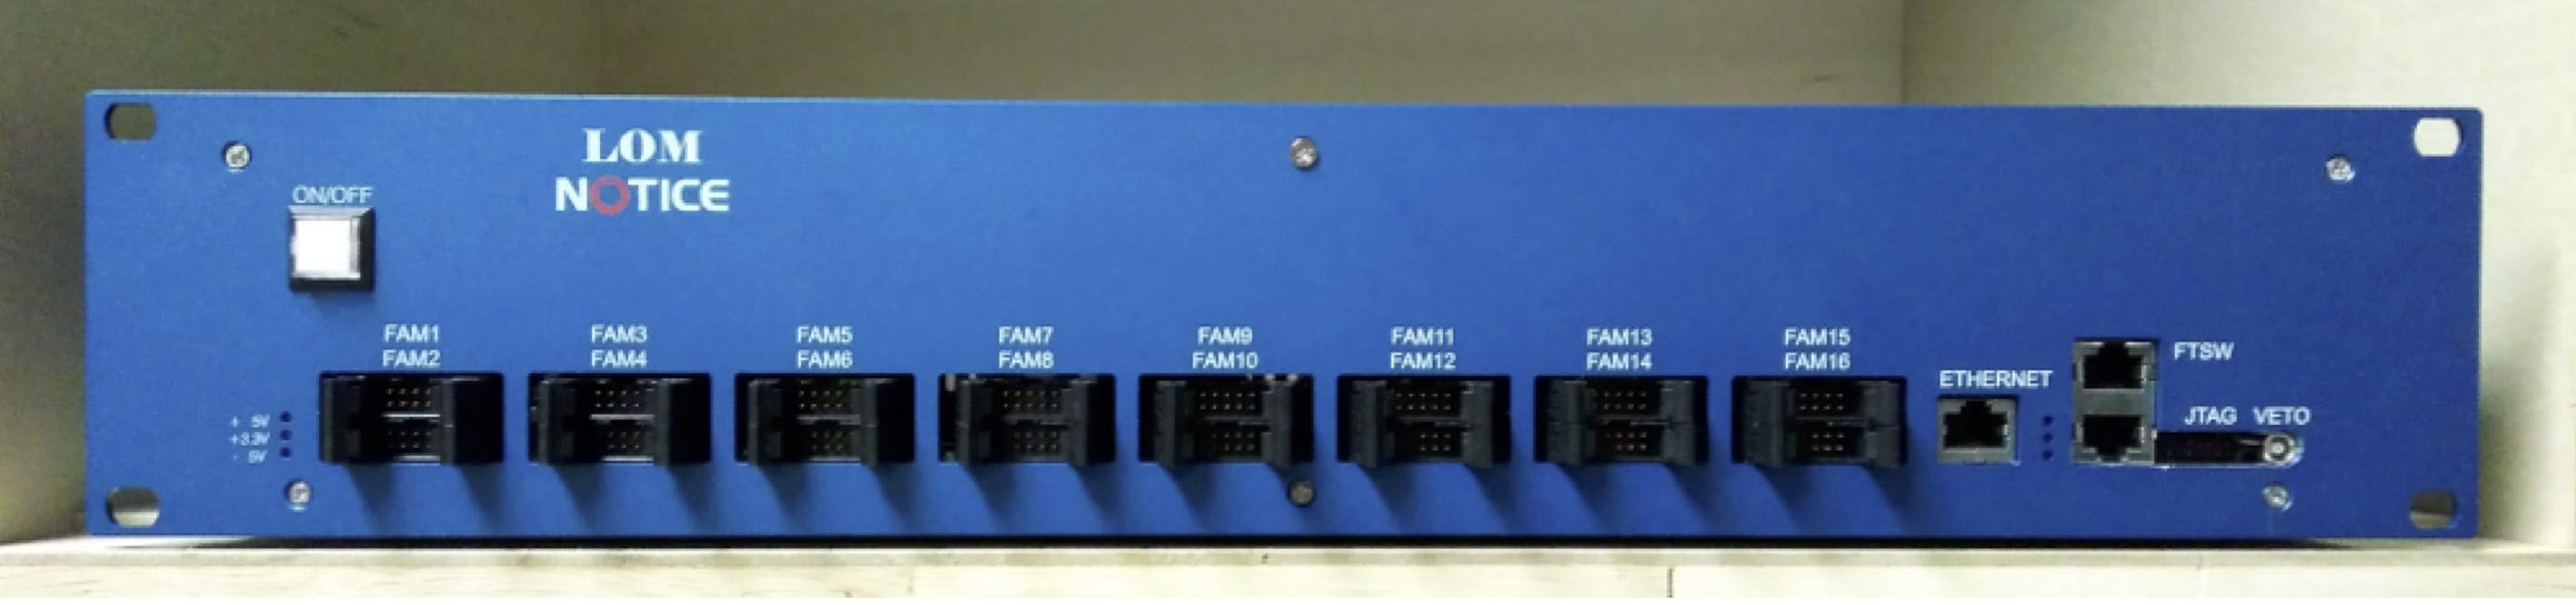
\includegraphics[width=\textwidth]{LOM_picture}
  \caption{Лицевая панель монитора светимости.}
  \label{fig:galaxy}
\end{figure}
Ключевой особенностью LOM является то, что данный модуль способен измерять светимость в абсолютных единицах, в отличие от двух других мониторов светимости, которые работают только в относительных единицах \cite{LumiBelle2}.\par 
  Монитор светимости направлен на измерение скорости счета $e^+e^-$ рассеяния с торцевых частей электромагнитного калориметра, произошедшего в коллинеарных секторах торцевых частей (Рис. 6).
\begin{figure}[htp]
  \centering
  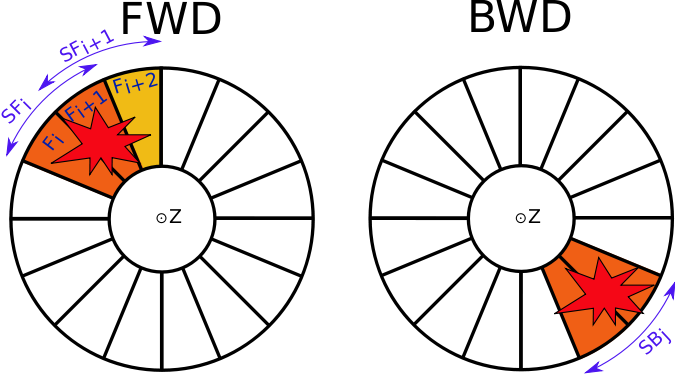
\includegraphics[width=0.5\textwidth]{lom_illustration.png}
  \caption{Схема энерговыделения в секторах при возникновении события $e^+e^-$ рассеяния.}
  \label{fig:galaxy}
\end{figure}
